\newpage
\maketitle
\begin{center}
\Large \textbf{第1章 时间序列基本特性} \quad 
\end{center}
\begin{abstract}
在本章中我们将讨论时间序列的基本特性,包括自相关性和平稳性。
\end{abstract}
\section{时间序列基本特性}
时间序列的自相关性是指时间序列过去与未来存在某种关系,是我们时间序列预测的基础。主要用自协方差函数(Autocovariance Function, AF)、自相关系数函数(Autocorrelation Coefficent Function, ACF)和偏自相关系数函数(Partial Autocorrelation Coefficient Function, PACF)来描述。
\subsection{随机变量统计量}
随机变量X其取值为$x$的均值定义为:
\begin{equation}
E(x) = \mu
\label{e000001}
\end{equation}
方差定义为:
\begin{equation}
\sigma ^{2} (x) = E\bigg[ \big( x - \mu \big)^{2} \bigg]
\label{e000002}
\end{equation}
其中$\sigma (x)$为标准差。
对于两个随机变量$x$和$y$,其协方差可以定义为:
\begin{equation}
\sigma (x, y) = E\bigg[ \big( x - \mu _{x} \big) \big( y - \mu _{y} \big) \bigg]
\label{e000003}
\end{equation}
在实际应用中,我们不可能知道真实的均值,只能使用统计量,因此协方差可以定义为:
\begin{equation}
Cov(x, y) = \frac{1}{n-1} \sum_{i=1}^{n} (x_{i} - \bar{x})(y_{i} - \bar{y})
\label{e000004}
\end{equation}
随机变量$x$和$y$的相关系数定义为:
\begin{equation}
\rho(x,y)=\frac{E[(x-\mu_{x})(y-\mu_{y})]}{\sigma _{x} \sigma _{y}}=\frac{\sigma(x,y)}{\sigma _{x} \sigma _{y}}
\label{e000005}
\end{equation}
采用统计量的表示方法为:
\begin{equation}
Cor(x,y)=\frac{Cov(x,y)}{std(x) \times std(y)}
\label{e000006}
\end{equation}
以上我们讨论的都是不同随机变量之间的关系,对于时间序列来说,我们可以把从不同时间点开始的子时间序列,视为不同的随机变量,那么我们就可以定义自协方差、自相关系数函数和偏自相关系数函数了。\newline
\subsection{时序序列平稳性}
时序信号$x_{t}$的均值定义为:
\begin{equation}
E(x_{t})=\mu (t)
\label{e000007}
\end{equation}
时间序列的均值与所考虑的时间点有关。我们可以把时间序列上每个时间点都视为一个独立的时间变量,但是对于时间序列而言,每个时间点的随机变量只有一个观测值,怎么求出均值呢?在实际应用中,我们会将时间序列中的趋势信号(上涨或下跌)、季节性信号等从时间序列中去除掉,对于剩下的残差序列,我们可以视为其各个时间点上的随机变量的均值是不变的,于是就可以使用下面的公式来计算均值:
\begin{equation}
\bar{x}=\frac{1}{N} \sum_{t=1}^{N}x_{t}
\label{e000008}
\end{equation}
由此我们引入平稳时间序列的概念,对于平稳时间序列,其各个时间点上对应的随机变量的均值相等。
时间序列的方差可以定义为:
\begin{equation}
\sigma ^{2}(t)=E[(x_{t}-\mu _t)^{2}]
\label{e000009}
\end{equation}
根据上面平稳时间序列的定义,各个时间点对应的随机变量的均值不变,则式\ref{e000009}可以化间为:
\begin{equation}
\sigma ^{2}(t)=E[(x_{t}-\mu)^{2}]
\label{e000010}
\end{equation}
我们同时规定,平稳时间序列各个时间点对应的随机变量的方差也不变,则\ref{e000010}可进一步化简为:
\begin{equation}
Var(x_{t})=\frac{1}{N-1} \sum_{t=1}{N} (x_t - \bar{x})^{2}
\label{e000011}
\end{equation}
\subsection{自协方差}
在讨论自协方差之前,我们首先要定义二阶平稳性。根据上一节定义,平稳时间序列是指各个时间点对应的随机变量的均值和方差相同。二阶平稳性是指在这一基础上,不同时间点对应的随机变量的相关系数只与时间相隔(lag)相关。注意:以下我们讨论的各种性质,均以此为前提。
对于lag=k的自协方差定义为:
\begin{equation}
C_{k}=E[(x_{t} - \mu)(x_{t+k} - \mu)]
\label{e000012}
\end{equation}
\subsection{自相关系数函数ACF}
由于自协方差的大小与随机变量的大小有关,无法准确衡量其间的关系,因此我们引入自相关系数函数ACF:
\begin{equation}
\rho _{k} = \frac{C_{k}}{\sigma ^{2}}
\label{e000013}
\end{equation}
由定义可知:
\begin{equation}
\begin{aligned}
\rho _{0} = \frac{C_{0}}{\sigma ^{2}} = \frac{E[(x_{t} - \mu)(x_{t} - \mu)]}{\sigma ^{2}} \\
= \frac{E[(x_{t} - \mu)^{2}]}{\sigma ^{2}} = \frac{\sigma ^{2}}{\sigma ^{2}} = 1\\
\end{aligned}
\label{e000014}
\end{equation}
在实际应用中,我们都是处理的离散数据点,则自协方差可以定义为:
\begin{equation}
c_{k}=\frac{1}{N}\sum_{t=1}^{N}(x_{t}-\bar{x})(x_{t+k} - \bar{x})
\label{e000015}
\end{equation}
自相关系数函数ACF可以定义为:
\begin{equation}
r_{k}=\frac{c_{k}}{c_{0}}
\label{e000016}
\end{equation}
\subsection{自相关性举例}
下面我们以上证综指时间序列为例,来看自相关系数函数ACF和偏自相关系数函数PACF的求法和作图,程序代码如下所示:
\lstset{language=PYTHON, caption={时间序列基本性质}, label={c000001}}
\begin{lstlisting}
import pandas as pd
import matplotlib.pyplot as plt
import matplotlib.dates as mdates
from matplotlib.font_manager import FontProperties
from statsmodels.tsa import stattools
from statsmodels.graphics import tsaplots

class Chp023(object):
    def __init__(self):
        self.name = 'Chp022'
        # 数据文件格式:编号 日期 星期几 开盘价 最高价 
        # 最低价 收益价 收益
        self.data_file = 'data/pqb/chp023_001.txt'
        
    def startup(self):
        print('第23章:时间序列基本性质')
        data = pd.read_csv(self.data_file, sep='\t', index_col='Trddt')
        sh_index = data[data.Indexcd==1]
        sh_index.index = pd.to_datetime(sh_index.index)
        sh_return = sh_index.Retindex
        print('时间序列长为:N={0}'.format(len(sh_return)))
        acfs = stattools.acf(sh_return)
        print(acfs)
        pacfs = stattools.pacf(sh_return)
        print(pacfs)
        tsaplots.plot_acf(sh_return, use_vlines=True, lags=30)
        plt.show()
        tsaplots.plot_pacf(sh_return, use_vlines=True, lags=30)
        plt.show()
\end{lstlisting}
数据文件格式为:
\begin{figure}[H]
	\caption{数据文件格式}
	\label{f000001}
	\centering
	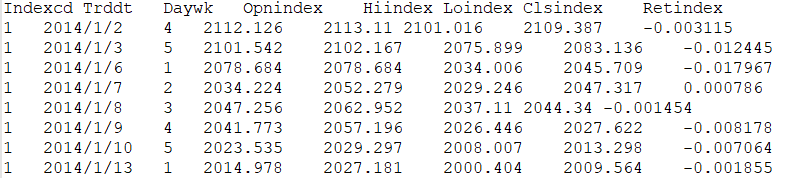
\includegraphics[height=3cm]{images/f000001}
\end{figure}
其运行结果为:
\begin{figure}[H]
	\caption{运行结果}
	\label{f000002}
	\centering
	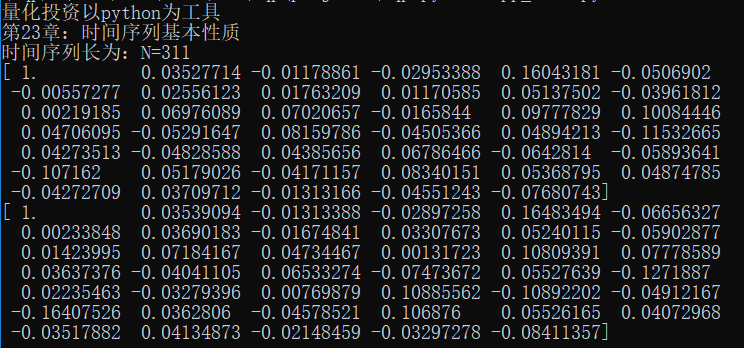
\includegraphics[height=3cm]{images/f000002}
\end{figure}
在图\ref{f000002}中,第一个数据为自相关系数函数ACF各期的值,而第二个数组为偏自相关系数函数PACF各期的值。判断时间序列是否具有自相关性,可以看除ACF和PACF中,除第一个元素外,有没有显著超过阈值的元素,阈值定义为:
\begin{equation}
threshold=\frac{1.96}{\sqrt{N}} = \frac{1.96}{\sqrt{311}} = 0.11
\label{e000017}
\end{equation}
式\ref{e000017}中的N为时间序列样本数,在本例中,共有311条记录,故N=311,所以其阈值为0.11左右。由于$acf[4]=0.16>0.11$所以可以推断其具有自相关性,同时$pacf[4]=0.165>0.11$也可以推断其具有自相关性。我们还可以通过图形的方式形像的表示出来,自相关系数函数图如所示:
\begin{figure}[H]
	\caption{自相关系数函数图}
	\label{f000003}
	\centering
	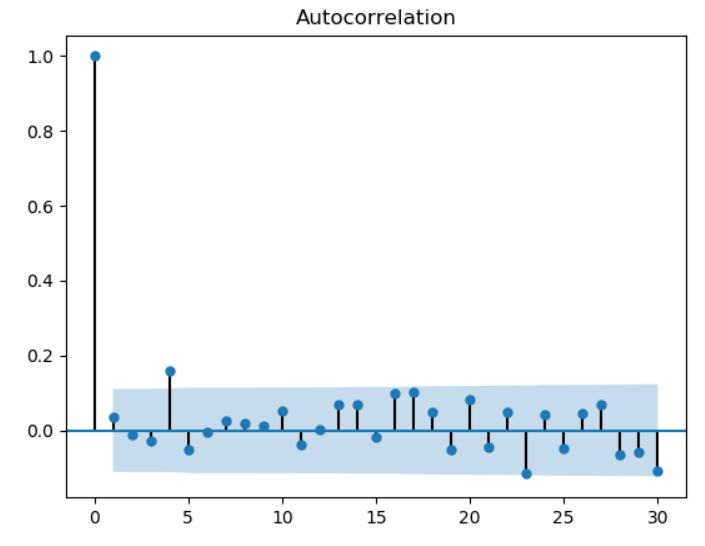
\includegraphics[height=4cm]{images/f000003}
\end{figure}
图\ref{f000003}中蓝色区域的界限为$[-\frac{1.96}{\sqrt{N}}, \frac{1.96}{\sqrt{N}}]=[-0.11, 0.11]$,除第1项外,其他项如果超出蓝色区域则说明此时间序列具有自相关性。\newline
偏自相关系数函数图为:
\begin{figure}[H]
	\caption{偏自相关系数函数图}
	\label{f000004}
	\centering
	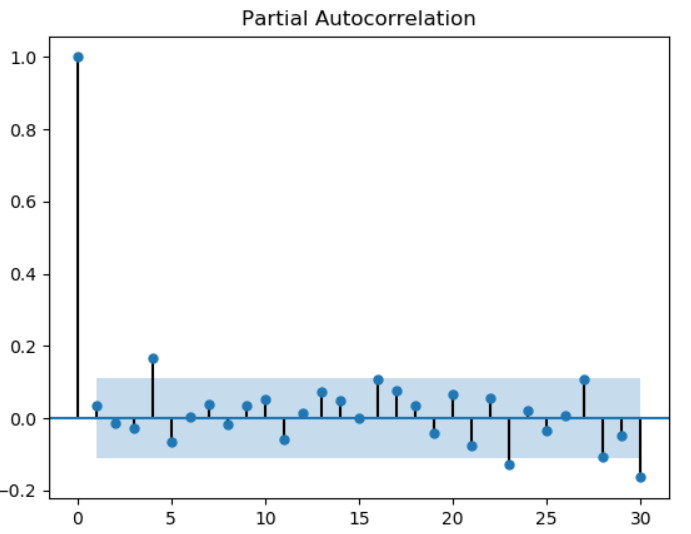
\includegraphics[height=4cm]{images/f000004}
\end{figure}
\subsection{白噪声和随机游走}
\subsubsection{残差序列定义}
我们要对任意时间序列$y_{t}$进行建模,我们的模型为$\hat{y}_{t}$,残差序列$x_{t}$可以定义为:$x_{t}=y_{t}-\hat{y}_{t}$,我们的任务就是使残差时间序列中每一个时间点对应的随机变量互相独立,没有自相关性,即满足独立同分布(Independent and Identical Distribution,I.I.D)条件。如果各个随机变量$x_{t} \sim \mathbb{N}(0, \sigma ^{2})$,则称其为高斯白噪声。\newline
\subsubsection{差分运算符}
为了后续讨论问题方便,我们首先定义BSO运算符:
\begin{equation}
Bx_{t}=x_{t-1} \quad B^{n}x_{t}=x_{t-n}
\label{e000018}
\end{equation}
我们定义差分运算符为:
\begin{equation}
\begin{aligned}
\nabla x_{t} = x_{t}-x_{t-1}=(1-B)x_{t} \\
\nabla x_{t}^{n} = \big( x_{t}-x_{t-n} \big)^{n}=(1-B)^{n}x_{t}
\end{aligned}
\label{e000019}
\end{equation}
\subsubsection{白噪声定义}
对于时间序列$\{ w_{t}, t=1,2,3,...,N \}$,满足$\forall t \quad w_{t} \sim \mathcal{N}(0, \sigma ^{2})$且$\forall i \ne j \quad Cor(w_{i}, w_{j})=0$,则其为白噪声时间序列。\newline
下面我们来看白噪声的二阶属性:
\begin{equation}
\begin{aligned}
\mu = E(w_{t})=0 \\
\gamma _{k}= Cor(w_{t}, w_{t+k}) = \begin{cases}
1 \quad if \quad k=0 \\
0 \quad if \quad k \ne 0
\end{cases}
\end{aligned}
\label{e000020}
\end{equation}
\subsubsection{随机游走}
随机游走(Random Walk)时间序列是指$x_{t}$可以定义为:$x_{t}=x_{t-1}+w_{t}$,其中$w_{t}$为白噪声时间序列。随机游走时间序列可以表示为:
\begin{equation}
\begin{aligned}
x_{t}=x_{t-1}+w_{t}=Bx_{t}+w_{t} \\
x_{t}=x_{t-1}+w_{t}=x_{t-2}+w_{t-1}+w_{t} \\
...... \\
x_{t}=w_{1} + w_{2} + ... + w_{t-1} + w_{t}
\end{aligned}
\label{e000021}
\end{equation}
所以随机游走时间序列可以看作是多个白噪声时间序列的叠加。下面我们来看随机游走时间序列的均值和协方差:
\begin{equation}
\begin{aligned}
\mu = 0 \\
\gamma _{k}(t)=Cov(x_{t}, x_{t+k})=t \sigma ^{2}
\end{aligned}
\label{e000022}
\end{equation}
我们再来看随机游走序列的自相关系数函数ACF:
\begin{equation}
\begin{aligned}
\rho _{k}(t)=\frac{Cov(x_{t}, x_{t+k})}{\sqrt{ Var(x_{t}) \cdot Var(x_{t+k}) }} \\
=\frac{t \sigma ^{2}}{\sqrt{t \sigma ^{2} (t+k) \sigma ^{2}}}=\frac{1}{\sqrt{1+ \frac{k}{t} }}
\end{aligned}
\label{e000023}
\end{equation}
在通常情况下,t比k要大得多,因此$\rho_{k}$会比较接近于1。\newline
下面我们来模拟一个随机游走时间序列信号,程序如下所示:
\lstset{language=PYTHON, caption={随机游走过程模拟}, label={c000003}}
\begin{lstlisting}
    def random_wale_demo(self):
        '''
        随机游走时间序列建模示例
        '''
        w = np.random.standard_normal(size=1000)
        x = w
        for t in range(1, len(w)):
            x[t] = x[t-1] + w[t]
        plt.plot(x, c='b')
        plt.title('Random Walk Demo')
        plt.show()
        acfs = stattools.acf(x)
        print(acfs)
        tsaplots.plot_acf(x, use_vlines=True, lags=30)
        plt.show()
        # 拟合随机游走信号
        r = []
        for t in range(1, len(x)):
            r.append(x[t] - x[t-1])
        rd = np.array(r)
        plt.plot(rd, c='r')
        plt.title('Residue Signal')
        plt.show()
        rd_acfs = stattools.acf(rd)
        print(rd_acfs)
        tsaplots.plot_acf(rd, use_vlines=True, lags=30)
        plt.show()
\end{lstlisting}
我们首先通过$x_{t}=x_{t-1}+w_{t}$生成一个随机游走信号,该信号图形如下所示:
\begin{figure}[H]
	\caption{随机游走时间序列信号}
	\label{f000005}
	\centering
	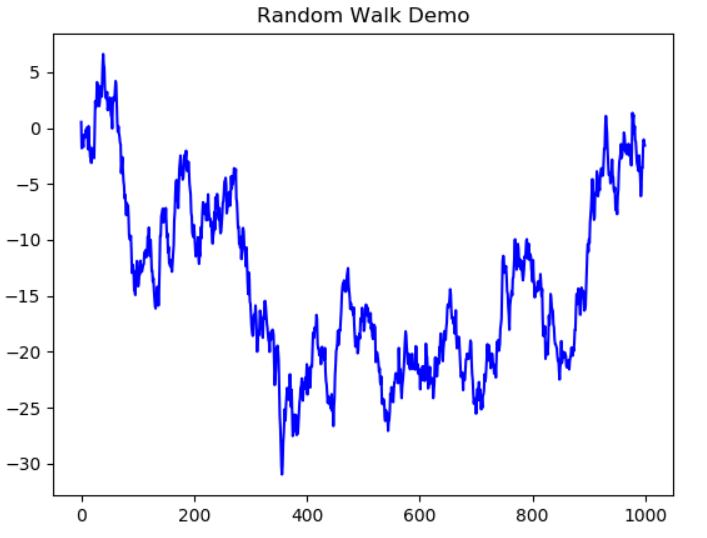
\includegraphics[height=5cm]{images/f000005}
\end{figure}
由图\ref{f000005}可以看出,其非常像是一个股票收盘价的走势图,这也是为什么有些人说股票走势是随机游走过程了。接着我们求出该时间序列的自相关系数函数ACF及其自相关图,如下所示:
\begin{figure}[H]
	\caption{随机游走时间序列信号}
	\label{f000006}
	\centering
	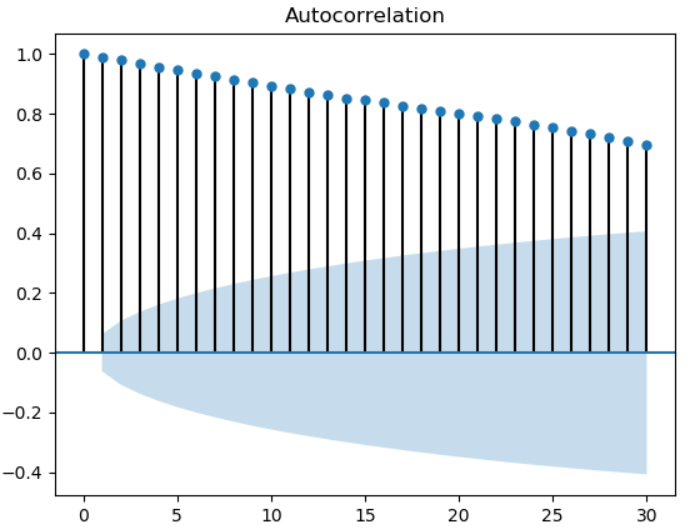
\includegraphics[height=5cm]{images/f000006}
\end{figure}
由图可以看出,其具有极强的自相关性,所有ACF值均位于蓝色置信区间之外。\newline
我们知道$x_{t}-x_{t-1}=w_t$,而$w_t$是白噪声时间序列信号,这实际上模拟了实际应用过程,我们把$x_t$视为实际的金融信号,而$x_{t-1}$为我们建模的信号,将两个信号相减,得到残差信号,如果残差信号是白噪声信号,就可以认为我们建模是合理的。下面来看我们得到的残差信号:
\begin{figure}[H]
	\caption{残差时间序列信号}
	\label{f000007}
	\centering
	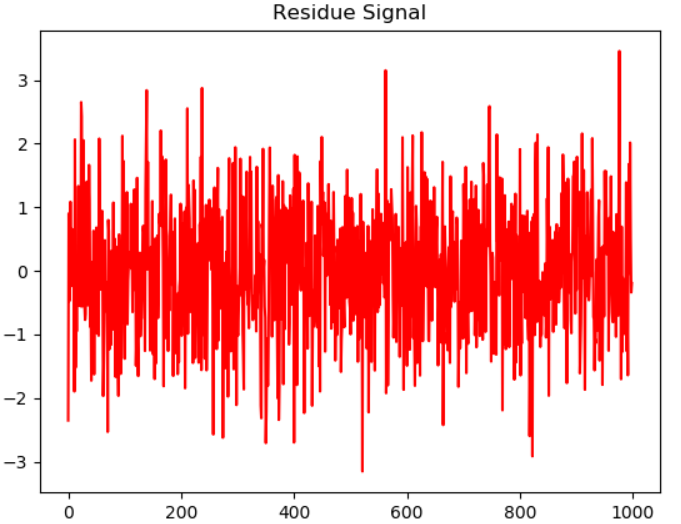
\includegraphics[height=5cm]{images/f000007}
\end{figure}
计算并绘制ACF如下所示:
\begin{figure}[H]
	\caption{残差自相关系数函数}
	\label{f000008}
	\centering
	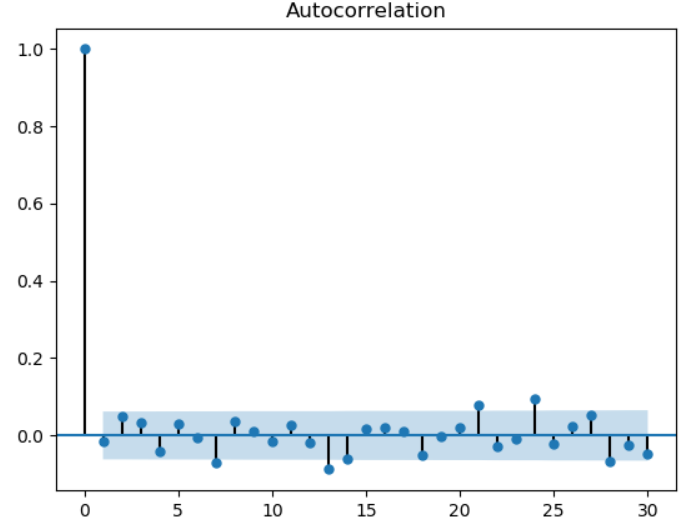
\includegraphics[height=5cm]{images/f000008}
\end{figure}
程序的运行结果如下所示:
\begin{figure}[H]
	\caption{程序运行结果}
	\label{f000009}
	\centering
	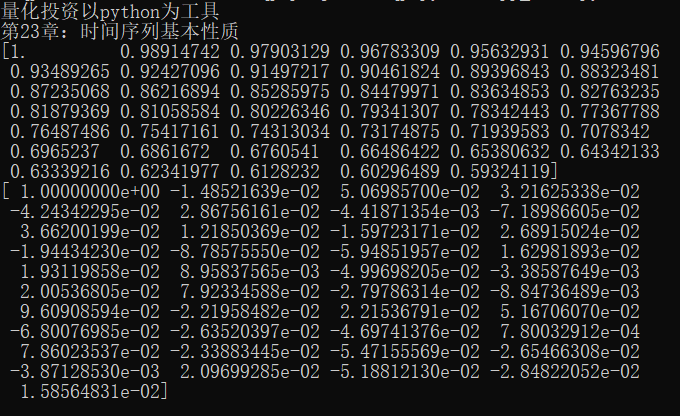
\includegraphics[height=5cm]{images/f000009}
\end{figure}
下面我们以上证综指收益率为例,来看随机游走模型是否可以很好的拟合这个时间序列,程序如下所示:
\lstset{language=PYTHON, caption={随机游走拟合上证综指收益率}, label={c000004}}
\begin{lstlisting}
    def random_walk_fit(self):
        data = pd.read_csv(self.data_file, sep='\t', index_col='Trddt')
        sh_index = data[data.Indexcd==1]
        sh_index.index = pd.to_datetime(sh_index.index)
        sh_return = sh_index.Retindex
        print('时间序列长为:N={0}'.format(len(sh_return)))
        r = []
        for t in range(1, len(sh_return)):
            r.append(sh_return[t] - sh_return[t-1])
        rd = np.array(r)
        plt.plot(rd, c='b')
        plt.title('Random Walk fit SHIndex Return')
        plt.show()
        rd_acfs = stattools.acf(rd)
        print(rd_acfs)
        tsaplots.plot_acf(rd, use_vlines=True, lags=30)
        plt.show()
\end{lstlisting}
其残差图像为:
\begin{figure}[H]
	\caption{残差图形}
	\label{f000010}
	\centering
	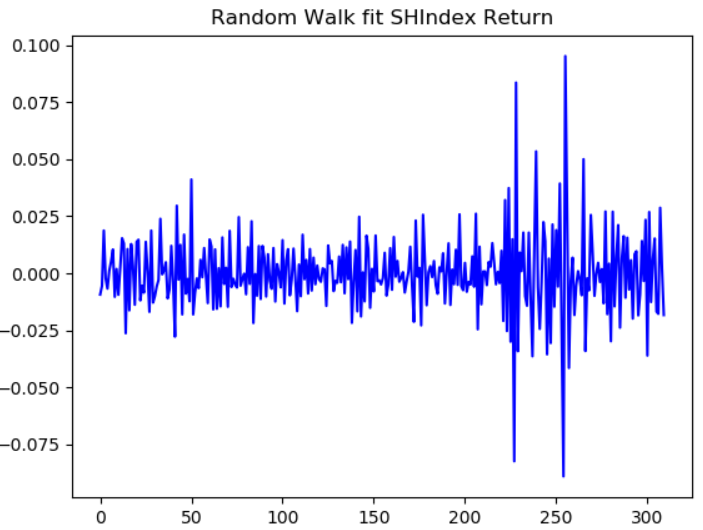
\includegraphics[height=5cm]{images/f000010}
\end{figure}
自相关系数函数ACF图形:
\begin{figure}[H]
	\caption{自相关系数函数ACF}
	\label{f000011}
	\centering
	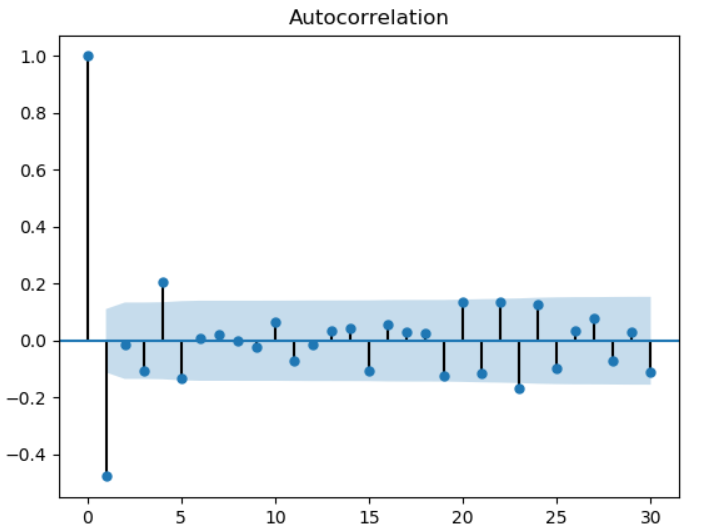
\includegraphics[height=5cm]{images/f000011}
\end{figure}
由图\ref{f000011}所示,在1、4时间点,明显超出置信范围,因此随机游走过程不能很好的拟合上证综指收益率时间序列信号。程序的运行结果如下所示:
\begin{figure}[H]
	\caption{程序运行结果}
	\label{f000012}
	\centering
	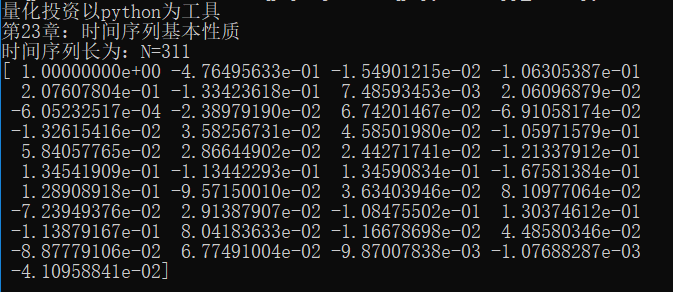
\includegraphics[height=5cm]{images/f000012}
\end{figure}